\documentclass[lettersize,journal]{IEEEtran}
\usepackage{amsmath,amsfonts}
\usepackage{algorithmic}
\usepackage{algorithm}
\usepackage{array}
\usepackage[caption=false,font=normalsize,labelfont=sf,textfont=sf]{subfig}
\usepackage{textcomp}
\usepackage{stfloats}
\usepackage{url}
\usepackage{verbatim}
\usepackage{graphicx}
\usepackage{cite}
\usepackage[hypcap=false]{caption}
\usepackage{float}

% Set path for images
\graphicspath{ {./images/} }

\newenvironment{Figure}
    {\par\medskip\noindent\minipage{\linewidth}}
    {\endminipage\par\medskip}


\begin{document}

\title{An Explainable Machine Learning Approach to Antenna Design}

\author{Tyler Carr \\ carrt12@my.erau.edu \\ Embry-Riddle Aeronautical University \\ Daytona Beach, FL}

\maketitle

\begin{abstract}
Antenna design process require extensive simulations tasks that are resource and time intensive, and are prone to interruptions. Furthermore, design equations are only available for predefined limited set of antenna geometries. By applying a machine learning algorithm to data that has already been generated from simulations of an antenna, performance metrics can be predicted significantly quicker than running full simulations. Insights about which geometric parameter had the most significant impact on the prediction can be drawn from the model and included in the output. Additionally, the model can be reversed so that for a particular form of antenna, an optimal geometry can be produced that will result in a specified performance. 
\end{abstract}

\section{Introduction}
Antenna designs require simulation in order to determine the performance of the antenna. Ansys High Frequency Simulation Software (HFSS) is an electromagnetic simulation software which is used to design and simulate the frequency of antennas. When designing the antenna, details such as dimensions of the antenna geometry, materials used for the antenna, and frequency are specified~\cite{Maxworth_2022}. Simulations are then run.


\subsection{Dataset}
The input to the simulation is a table that consists of every combination of the varying values of each dimension, with each dimension having a set range and a certain value that it is incrementing by. This is also associated with a frequency value. Each combination is associated with a particular S11 value. S11 value are used as a measure of performance. An S11 value, also known as the reflection coefficient, represents the amount of power reflected from the antenna. An example of an S11 value is 0dB, which would mean that all of the power is being reflected from the antenna, meaning that there is no radiation. Ideally, this value should be below -10dB~\cite{Bevelacqua_2015}.


\subsection{Simulation Issues}
The main issue with running simulations in HFSS is the amount of time that it takes. The matrix operations that are required to run many iterations of simulations to analyze loss can take multiple days to complete~\cite{john_antenna_2009}. Depending on how the simulation is set up, this process could be impacted by power outages or software bugs, resulting in a loss of data and requiring manual intervention to re-run the simulation. 

HFSS works by specifying a range of dimensions and outputting performance metrics, such as S11 values. This is insightful, but there is a degree of trial and error involved in finding an optimal antenna geometry. One would start by specifying what they would think would be the ideal antenna geometry using their own intuition. Based on the results from an initial simulation run, geometry values would be adjusted in an attempt to optimize the geometry.

By using a machine learning algorithm to do the bulk of the investigative work, the amount of simulation iterations that need to be run to optimize an antenna's geometry can be significantly reduced. The algorithm can then be used to fill in the missing gaps between the reduced data with estimates, making it easier to narrow down to a specific area of interest. 

\subsection{Reversing the Problem}
After training a machine learning model on the dataset, a table is produced with significantly more rows than was started with from the simulated data. Predictions can be searched by specifying the desired S11 value and a range of frequency values that the antenna should operate between. Antenna geometries that match the search are returned, which saves significant time that would be required to set up and perform additional simulations. When seeking an optimal geometry between a certain frequency range, the geometry that results in the S11 with the lowest maximum S11 range would be chosen.

\section{Related Work}
Machine learning topics with antenna design optimizations have been explored before. The algorithm and methods that are chosen ultimately depend on the way that the antenna geometry is expressed. One format that the input data can have is to be in tabular format, where rows represent combinations of geometry measurements and some performance specification, such as S11. For rows of data, algorithms that have been used before can be something like a Artificial Neural Networks, Gaussian Network, or Gaussian Process Regression. The other type of format that the input data can have would be where the geometry is represented with pixels with a matrix of integers each representing a different material being used. This second format is useful for Convolutional Neural Networks and allows for exploring new antenna geometry designs instead of only staying within predefined restrictions.~\cite{wu_machine_2023} 


\section{Methodology}
In order to determine the optimal antenna geometry, a machine learning algorithm was employed. This algorithm is trained with a supervised learning method on a preexisting dataset. This dataset came from a parametric sweep performed in HFSS on the simulated antenna design. In this input data, each row represents a combination of geometry dimensions, frequency, and an associated S11 value. The features, or independent variables, of this problem are the geometry dimensions and frequency. The targets, or dependent variables, are the S11 values. 

Previously, small increments of data would have to be simulated by the parametric sweep and manually inspected for performance, which takes a lot of time to perform. Training the machine learning model on data with larger increments allows for a shorter simulation time, since the model will fill in the gaps with predictions. It also aids in providing a better guess of an optimal algorithm for a particular performance, helping optimize the antenna faster. 

For the development of the algorithm, a Grounded CPW Leaky Wave Antenna was used. This is a new antenna design being developed by a student that needed optimization.

\subsection{Analyzing the Data}
In order to determine if a S11 value was predicted accurately, a tolerance was utilized. An exact prediction of an S11 value down to multiple decimal points of precision is very unlikely, so this tolerance allows allows for some flexibility. The tolerance is the error that we allow the value to contain, and we consider the prediction accurate if it is within the range above or below the true value. The tolerance is important for an accurate model, and ideally this value should be below one.

A regression algorithm was chosen as the target is numeric. 20\% of the dataset provided by the parametric sweep was reserved for testing and comparing the performance of the models, and the remainding 80\% was used to train the models. Two common metrics to compare algorithm performance are to use the R-square score~\eqref{eq:rsquared} and the RMSE (Root Mean Squared Error)~\eqref{eq:rmse} when comparing the simulated and predicted S11 values~\cite{haque_machine_2023,m_el-kenawy_optimized_2022}. 

\begin{figure}
    \begin{equation}
        R^2 = 1 - \frac{\text{SSR}}{\text{SST}}
        \label{eq:rsquared}
    \end{equation}
    \begin{equation}
        {RMSE} = \sqrt(\frac{1}{n} \sum_{i=1}^{n}(y_i - \hat{y}_i)^2)
        \label{eq:rmse}
    \end{equation}
    \caption{Formulas for R-squared and RMSE}
\end{figure}



\subsection{Preprocessing}
Preprocessing is a necessary step with any data being processed through a machine learning algorithm. Only after the data is preprocessed will it yield beneficial results from the algorithm. 

The first step was to exclude any data that was considered invalid. Data points with S11 values that are greater than zero are ignored. This should never happen in a real scenario, and if this occurs, it means that there was an error with the calculation. 

The next preprocessing action that was performed was scaling. This process linearly transforms the ranges of the geometry parameters to have the same scale. This is performed so all features are weighted the same and no one feature is artificially weighted more than the others. 

\subsection{TensorFlow}
TensorFlow was used to create a deep neural network with multiple layers in order to make predictions of the S11 value.

The hyperparameters were tuned in an attempt to both improve the accuracy and reduce the error rate of the model. This was done by adjusting various hyperparameters of the model, including the number of layers in the network, the rate at which the model learns, andw the unit of each layer, which represents the number of neurons and outputs. This was done using a randomized searching method. In typical grid search hyperparameter tuning, the search space grows too large to be feasibly tested fairly quickly. With the randomized search method, a random subset of hyperparameter combinations can be tested. The most optimal results are not guaranteed, but it can get relatively close~\cite{omalley2019kerastuner}. 

TODO write about gpu and cpu, what metrics were used, what graphs were generated 

\subsection{Scikit-learn}


TODO write about all models tested, how the preprocessing was the same insert graphs and talk about them 

\subsection{Finding Optimal Geometry}
TODO write about methods used comparing sklaern, tensorflow


\begin{Figure}
\centering
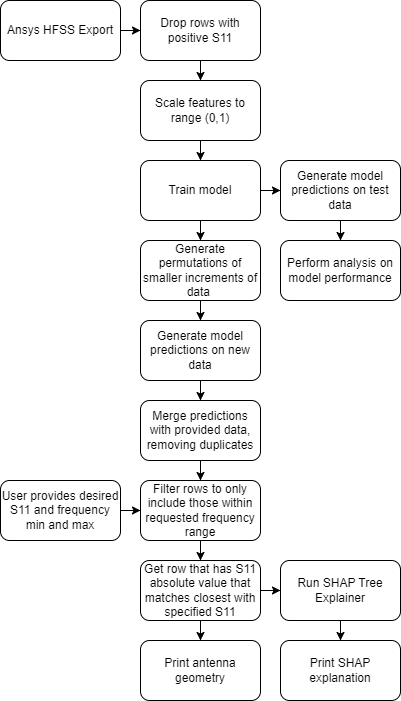
\includegraphics[width=3.0in]{methodology}
\captionof{figure}{Flow of data through the system}
\label{data_flow}
\end{Figure}


\section{Results}
All of the following were performed on the same machine to eliminate the possibility of hardware anomalies. The machine that was used contained a  Intel\textregistered~Core\texttrademark~i9\-10900X CPU @ 3.70GHz and a NVIDIA GeForce RTX 3090 graphics card. 

\subsection{Library and Model Comparison with Leaky Wave Antenna}
The Leaky Wave Antenna was used to test and compare the performance of models from the two different libraries: TensorFlow and Scikit-learn. The best performing model was chosen from each library, and their training time, predicting time, accuracy, and RMSE were compared in order to select the best model.

The Keras Tuner search for optimal hyperparameters of the DNN (deep neural network) provided the results in Table~\ref{keras_best_params}. It found that the model performed best with the maximum number of layers out of the testing range, and the optimal learning rate was in the middle of the testing range. This DNN was only able to predict S11 values with an error tolerance of~$\pm$1 with a 31.75\% accuracy. This low accuracy gives the hint that this might not be the best model for the job.

Figure \ref{dnn_loss_graph} shows how the DNN's loss decreased as the number of epochs increased. The fact that this graph shows both the training and testing decreasing shows that the model is converging. Additionally, the model is not overfitting. 

\begin{table}[h]
\caption{Keras Tuner Best Hyperparameters}
\begin{center}
\begin{tabular}{ |c|c|c| }
    \hline
    Hyperparameter Name & Hyperparameter Value \\ 
    \hline
    num\_layers & 4 \\  
    \hline
    units\_0 & 256 \\
    \hline
    units\_1 & 32 \\
    \hline
    units\_2 & 32 \\
    \hline
    units\_3 & 32 \\
    \hline
    learning\_rate & 0.011724 \\
    \hline
\end{tabular}
\end{center}
\label{keras_best_params}
\end{table}

\begin{Figure}
    \centering
    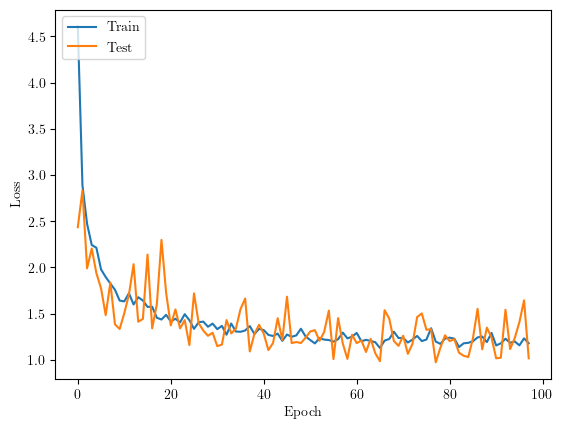
\includegraphics[width=2.5in]{loss}
    \captionof{figure}{DNN Loss Graph}
    \label{dnn_loss_graph}
\end{Figure}

TODO insert tensorflow epoch vs accuracy +- 1 graph? 

TODO insert data about sklearn 

When comparing the TensorFlow and Scikit-learn libraries, the same random state was used when splitting the data into training and testing portions. This ensures that each library is given a fair chance with the same set of data and the data isn't being swayed unintentionally. 

It's clear from the Table~\ref{comparing_libraries} that Scikit-learn is the best choice of library for this problem. The Scikit-learn model performed with 28.42\% better accuracy when predicting values with a tolerance of~$\pm$1. It trains and predicts significantly faster, and it has a lower RMSE.

\begin{table}[h]
\caption{Comparing Libraries}
\begin{center}
\begin{tabular}{ |c|c|c| }
    \hline
    Model Type & TensorFlow & Scikit-learn \\ 
    \hline
    Training Time (ms) & 25500 & 8.2 \\  
    \hline
    Predicting Time (ms) & 86.7 & 3.65 \\
    \hline
    S11 Accuracy within~$\pm$1 & 0.3175 & 0.60166 \\
    \hline
    RMSE & 16.7987 & 9.4661 \\
    \hline
\end{tabular}
\end{center}
\label{comparing_libraries}
\end{table}

TODO EXPLAIN BOTH THESE GRAPHS
Both show how sklearn is better for this problem

\begin{Figure}
    \centering
    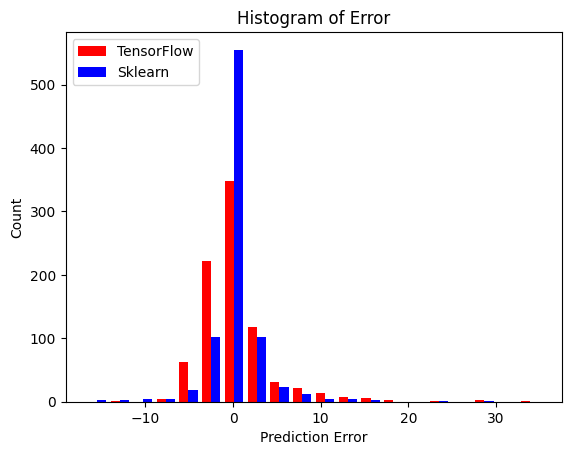
\includegraphics[width=2.5in]{histogram}
    \captionof{figure}{Histogram of Error}
    \label{historgram_of_error}
\end{Figure}

\begin{Figure}
    \centering
    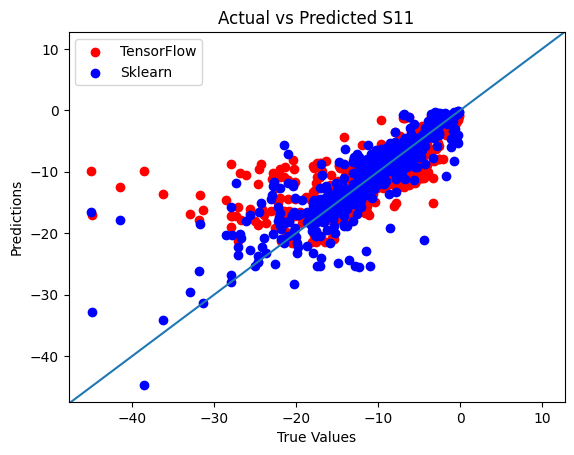
\includegraphics[width=2.5in]{actual_vs_predicted_s11}
    \captionof{figure}{Actual vs Predicted S11}
    \label{actual_vs_predicted_s11}
\end{Figure}

\subsection{Testing with Completely Unseen Data}
The chosen model was given a set of 3 geometries that had never been seen before by either the training set or testing set. They 

TODO FIX ME 


\section{Conclusion}

TODO CITE CAMERON for data
TODO cite TensorFlow


\bibliographystyle{IEEEtran}
\bibliography{refs}

\vfill

\end{document}